\documentclass[a4paper,11pt]{article}
\input{/home/tof/Documents/Cozy/latex-include/preambule_lua.tex}
\newcommand{\showprof}{show them}  % comment this line if you don't want to see todo environment
\fancyhead[L]{Réseau physique}
\newdate{madate}{10}{09}{2020}
\fancyhead[R]{Seconde - SNT} %\today
\fancyfoot[L]{~\\Christophe Viroulaud}
\fancyfoot[C]{\textbf{Page \thepage}}
\fancyfoot[R]{\includegraphics[width=2cm,align=t]{/home/tof/Documents/Cozy/latex-include/cc.png}}

\begin{document}
\begin{Form}
\paragraph{Objectif:}Comparer les différents modes de connexion au réseau internet.
\begin{commentprof}
\noindent\textbf{MATÉRIEL:} câble coaxial, câble Ethernet, fibre optique?\\
\end{commentprof}
\section{Modes de connexion}
\begin{framed}
\textbf{coaxial:} Le principe est de faire circuler le signal électrique dans le fil de données central. On se sert du maillage de masse pour avoir un signal de référence à 0V. On obtient le signal électrique en faisant la différence de potentiel entre le fil de données et la masse. Le câble 10B2 possède les caractéristiques suivantes:
\begin{itemize}
\item le 10 indique le débit en Mb/s (mégabits par seconde),
\item le B indique la façon de coder les 0 et les 1, soit ici la bande de Base,
\item le dernier chiffre indique la taille maximale du réseau, exprimée en mètres et divisée par 100.
\end{itemize}
\end{framed}
\begin{framed}
\textbf{Ethernet:} Il est composé de 4 fois 2 paires de fils torsadés. La différence de potentiel entre les 2 fils d'une même paire permet de transporter le signal. Nous utilisons 2 paires de fils: une pour envoyer les données, l'autre pour les recevoir. Le débit peut aller de 10 à 1000 mégabits par seconde selon le câble. On les branche à l'aide de prise RJ45. Nous rencontrons des diminutions de débit au delà de 100 mètres.
\end{framed}
\begin{framed}
\textbf{ADSL:} C'est une technologie qui permet de faire passer des données numériques par la paire de fils de cuivre d’une ligne téléphonique. Ces données sont transmises et reçues indépendamment du service téléphonique (voix) grâce à un filtre branché sur la prise. On considère qu’avec l’ADSL, un utilisateur métropolitain bénéficie d’un débit de l’ordre de 8 Mb/s pouvant atteindre 20Mb/s avec l'ADSL2+.
\end{framed}
\begin{framed}
\textbf{Fibre optique:} Une fibre optique est un fil dont l’âme, très fine, en verre ou en plastique, a la propriété de conduire la lumière et sert pour la transmission de données numériques. Les fournisseurs promettent un débit pouvant atteindre 1 Gbit/s (gigabits par seconde) avec un affaiblissement négligeable par rapport aux autres technologies. Théoriquement il est possible d'obtenir un débit de 100Gb/s.
\end{framed}
\begin{framed}
\textbf{WIFI:} La norme IEEE 802.11 est un standard international décrivant les caractéristiques d'un réseau local sans fil (WLAN). Grâce au Wi-Fi, il est possible de créer des réseaux locaux sans fils à haut débit pour peu que l'ordinateur à connecter ne soit pas trop distant du point d'accès (la box). La norme IEEE 802.11n annonce un débit théorique de 450Mb/s pour une portée de 250m. Ces chiffres sont à relativiser car très dépendants des infrastructures (mur, béton, colline...).
\end{framed}
\begin{framed}
\textbf{Bluetooth:} Bluetooth est une norme de communication permettant l'échange bidirectionnel de données à très courte distance en utilisant des ondes radio UHF sur une bande de fréquence de 2,4 GHz. Sa destination est de simplifier les connexions entre les appareils électroniques en supprimant des liaisons filaires.
\end{framed}
\begin{framed}
\textbf{4G:} La 4G désigne la quatrième génération de réseaux mobiles. Elle a succédé à la 3G. Chaque génération améliorant les performances, la 4G permet de surfer jusqu'à 10 fois plus vite qu’en 3G+ avec un débit maximum théorique de 75 ou 150 Mb/s. Les avantages de la 4G sont directement liés à l'accès data sur un appareil mobile. Le déploiement des antennes relais assure une couverture du territoire variant entre 80 et 90\% selon les opérateurs.
\end{framed}
\begin{framed}
\textbf{USB:} Le terme anglais \emph{Universal Serial Bus} ou USB est une norme relative à une connectique informatique en série qui sert à connecter des périphériques informatiques à un ordinateur ou à tout type d'appareil prévu à cet effet (tablette, smartphone, etc...). Les performances de l'USB, notamment concernant les débits, se sont grandement améliorées au fil des versions : de 1,5 Mbit/s pour la version 1.0 à 20 Gbit/s théoriques pour la version 3.2.
\end{framed}
\begin{commentprof}
certains types de connexion ne sont pas utilisés pour établir un réseau; certains sont obsolètes.
\end{commentprof}
\subsection{La bonne connexion}
\begin{figure}[!h]
\centering
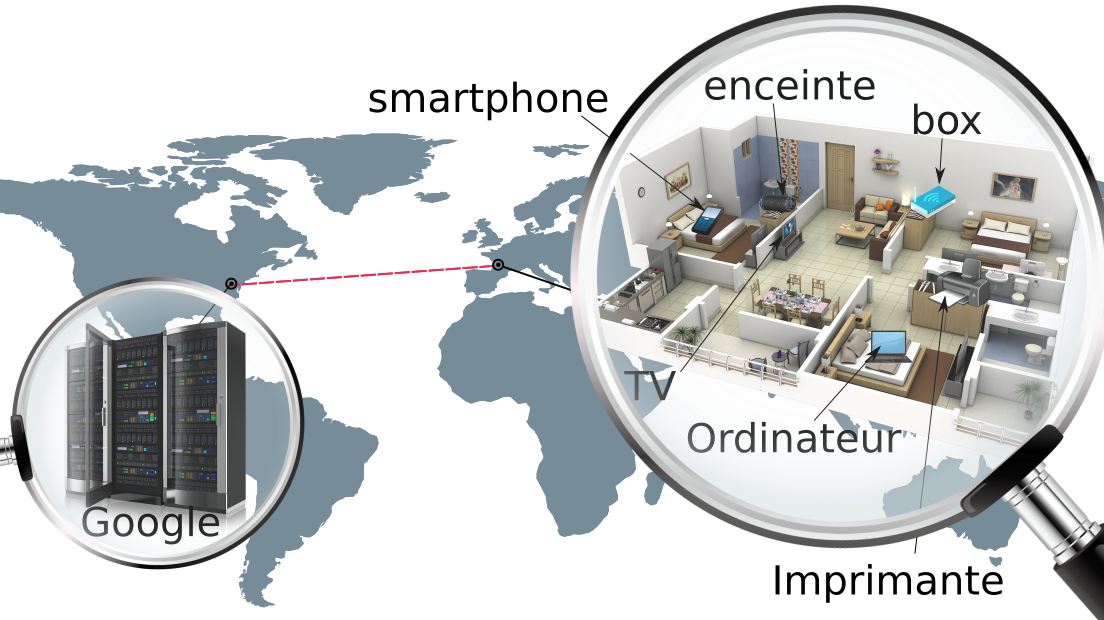
\includegraphics[width=17cm]{ressources/bonne-connexion.png}
\captionof{figure}{connexion}
\label{connexion}
\end{figure}
\begin{activite}
\begin{enumerate}
\item En s'aidant de la figure \ref{connexion} citer le(s) mode(s) de connexion adapté(s) aux différentes relations:
\begin{itemize}
\item smartphone $\longleftrightarrow$ internet
\item smartphone $\longleftrightarrow$ enceinte
\item ordinateur $\longleftrightarrow$ internet
\item télévision $\longleftrightarrow$ internet
\item imprimante $\longleftrightarrow$ ordinateur
\item box $\longleftrightarrow$ serveur Google
\end{itemize}
\item Citer ceux qui sont utilisés pour le réseau local.
\item Citer ceux qui sont utilisés pour le réseau internet.
\end{enumerate}
\end{activite}
\subsection{Débit}
Le débit se mesure en bits par seconde (noté b/s ou bps). On utilise plus fréquemment ses dérivés: le mégabits par seconde (Mb/s) ou le gigabits par seconde (Gb/s).
\begin{activite}
\begin{enumerate}
\item Convertir 100Gb/s en Mb/s.
\item Classer les modes de connexion dans l'ordre croissant de débit.
\item Quel type de connexion est-il préférable d'utiliser pour mettre en place les câbles reliant les continents. Justifier.
\end{enumerate}
\end{activite}
\subsection{Identifier les modes de connexion}
Certains protocoles d'internet permettent de gérer les changements de réseaux des appareils mobiles.
\begin{activite}
Dans la courte histoire ci-après, déterminer les types de connexions possibles d'Alice.
\begin{itemize}
\item 10h45: Depuis son appartement Alice envoie un mail à Bob pour lui proposer de déjeuner chez Burger King. Il répond dans l'instant et lui donne rendez-vous sur place à 12h30.
\item 12h15: Alice part de chez elle. En marchant dans la rue commerçante, elle aperçoit une paire de chaussures dans une vitrine. Avec son smartphone elle effectue une recherche web pour voir si elle peut l'acheter en ligne à un prix plus compétitif.
\item 12h41: Alice marche rapidement. Elle est encore à 300m du Burger King. Elle décide d'appeler Bob via WhatsApp, pour la prévenir de son retard. Tout en continuant sa conversation, elle rentre dans le restaurant et demande à Bob où il se trouve.
\end{itemize}
\end{activite}
\section{Trafic internet}
\subsection{Développement du trafic}
Chaque mois il s'échange sur internet de l'ordre de 168 millions de téraoctets de données. En 1990, ce chiffre était seulement de l'ordre de 1 téraoctet.\\1 téraoctet représente 1000 milliards d'octets.
\begin{activite}
Étudier les documents ou les pages web du diaporama \emph{trafic internet} sur le site \url{https://cviroulaud.github.io} puis répondre aux questions suivantes:
\begin{enumerate}
\item Que représente la première représentation graphique?
\item Quelle tendance exprime-t-elle?
\item Par quelle méthode se connecte-t-on majoritairement sur internet en 2017?
\item Quel(s) mode(s) de connexion est-il alors intéressant de développer?
\item Quel nouveau mode de connexion entend-on parler dans les médias récents et qui confirme la réponse à la question précédente?
\item Quels continents sont majoritairement interconnectés par le réseau internet?
\item Le câble le plus long du monde part de la pointe britannique, traverse la mer Méditerranée l'Égypte et la mer Rouge. Il rejoint l'Inde contourne le Sri Lanka et se termine au Japon. Quel est le nom de ce câble? Quelle est sa longueur?
\item Combien de câbles Google a-t-il déjà installé?
\item Quel et l'intérêt pour une entreprise comme Google de déployer un câble privé?
\end{enumerate}
\end{activite}
\subsection{Quels usages?}
\guill{L'Internet des objets (en anglais Internet of Things ou \textbf{IoT}) est l'interconnexion entre internet et des objets, des lieux et des environnements physiques. L'appellation désigne un nombre croissant d'objets connectés à internet permettant ainsi une communication entre nos biens dits physiques et leurs existences numériques.} \emph{de Wikipedia}
\begin{activite}
Étudier les documents du diaporama \emph{trafic internet}, lire les articles sur les sites proposés puis répondre aux questions suivantes:
\begin{enumerate}
\item Combien y-a-t-il de recherches effectuées sur le moteur Google en 1 minute?
\item Citer cinq objets autres qu'un ordinateur ou smartphone, qui peuvent se connecter au réseau internet.
\item Quelle conséquence le développement des IoT entraîne-t-il sur l'adressage IPv4?
\item Définir le terme \emph{smarthome}.
\item Quelle est la croissance du chiffre d'affaire des objets connectés entre 2017 et 2018?
\item Que peut-on supposer à propos de cette croissance pour les années suivantes?
\item Quel type de contenu est principalement consommé sur internet?
\item Quelle proportion du trafic internet mondial représente Netflix?
\end{enumerate}
\end{activite}
\end{Form}
\end{document}